% SVN info for this file
\svnidlong
{$HeadURL$}
{$LastChangedDate$}
{$LastChangedRevision$}
{$LastChangedBy$}

\chapter{Appendix}
\labelAppendix{appendix}

\begin{introduction}
  
\end{introduction}

\section{User Acceptance Testing}

%\lettrine[nindent=-1pt]{T}{REST API for BMI} is defined as the following:
\lettrine[nindent=-1pt]{U}{ser Acceptance Testing} \index{User Acceptance Testing (UAT)}implementation has been added to BMI in order validate a deployment through a black-box end-to-end system test.  This performs a \index{Behavior-Driven Development (BDD)}\emph{Behavior-Driven Development} scenario using the \code{behave}\footnote{\link{http://pythonhosted.org/behave/}} Python package.  

\subsection{Behavior-Driven Development (BDD)}

Behavior-Driven Development is defined through a live-document implemented using the Gherkin language\footnote{\link{https://github.com/cucumber/cucumber/wiki/Gherkin}}. which utilizes \emph{Given-When-Then} control-flow syntax defined as follows: \\

\begin{itemize}
\item[\code{Given }$\blacktriangleright$\hspace{-12mm}] \hspace{10mm}\emph{Defines a given state.}
\item[\code{When }$\blacktriangleright$\hspace{-12mm}] \hspace{10mm}\emph{Defines a given action performed under the given state.}
\item[\code{Then }$\blacktriangleright$\hspace{-12mm}] \hspace{10mm}\emph{Defines the expected outcome after the action is performed.} \\
\end{itemize}

In Figure \ref{fig:bdd-bmi-end-to-end-template} is defined the end-to-end test performing a scenario of steps, where each line is a step that refers to a function.

\pagebreak

\begin{figure}[!h] % Example of including images
%\label{fig:ceph-imported-cloned-image}
\begin{center}
%\includegraphics[width=0.5\linewidth]{#1}
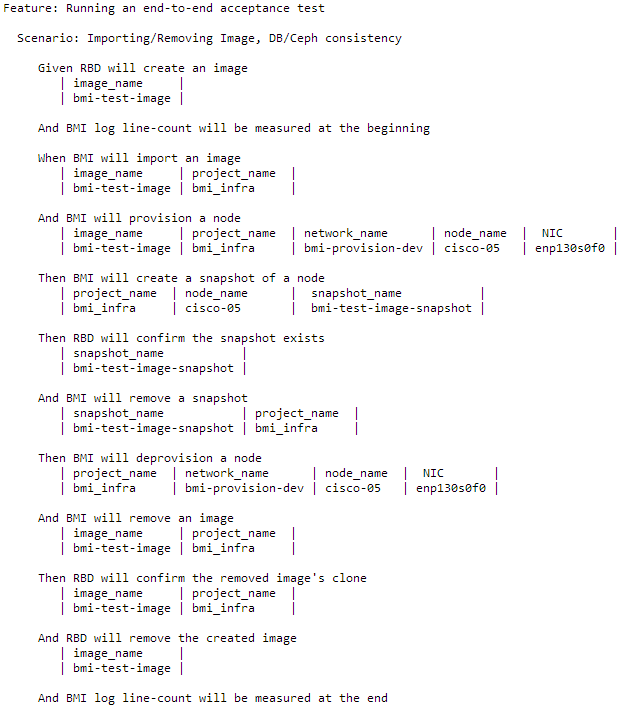
\includegraphics[scale=1]{figures/end-to-end-bdd-template.png}
\end{center}
\caption{The BMI End-to-End Behavior-Driven Deployment Test, with tables of parameters to test with.}
%\label{fig:example_figure}
\label{fig:bdd-bmi-end-to-end-template}
\end{figure}

For example, in Figure \ref{fig:bdd-bmi-function-definition} the creation of an RBD image at the start is defined through the \code{rbd\_create\_image()} function, where it is decorated by the sentence referenced in the live-document.

%\pagebreak

\begin{figure}[!h] % Example of including images
%\label{fig:ceph-imported-cloned-image}
\begin{center}
%\includegraphics[width=0.5\linewidth]{#1}
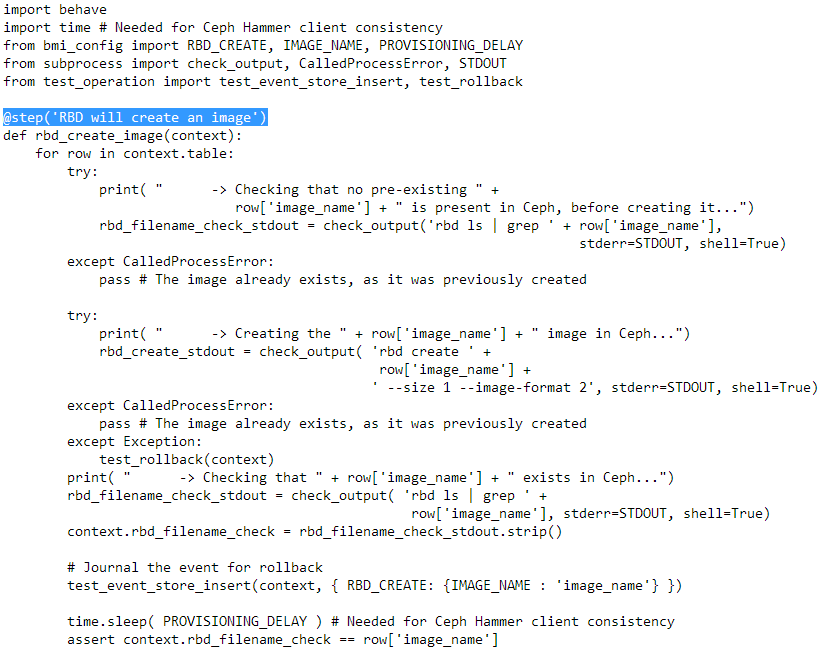
\includegraphics[scale=1]{figures/bmi-bdd-step-definition-v3.png}
\end{center}
\caption{The definition of the RBD creation step, where the decoration highlights the sentence referenced in the end-to-end deployment test}
%\label{fig:example_figure}
\label{fig:bdd-bmi-function-definition}
\end{figure}
\text{}\vspace{10mm}
\pagebreak

\subsection{Configuring the Acceptance Tests  \\ }

\index{configuring User Acceptance Tests}Before running the acceptance tests, it is necessary to configure BMI service to test.  This is performed by the following steps:

\begin{enumerate}

\item Copy the \code{acceptance-tests} directory to the new environment. \\
\item Proceed to the \code{config/tests-uat} directory and duplicate recursively one of the configuration, as such: \\

\code{     cp -r neu-haas-dev NEW\_BMI\_SERVICE\_TO\_TEST} \\

\pagebreak

   Example: \\

\code{     cp -r neu-haas-dev prb-bu-dev} \\

\item Enter the newly created directory and update the \code{config} file accordingly.  Below is an example of one: 

\code{
\text{}\hspace{6mm}   \\
\text{}\hspace{6mm}        export BMI\_RELEASE\_NAME=moc-0.5-release \\
\text{}\hspace{6mm}   \\
\text{}\hspace{6mm}        export BMI\_PROJECT=bmi\_infra \\
\text{}\hspace{6mm}        export HIL\_NODE=cisco-05 \\
\text{}\hspace{6mm}        export HIL\_NETWORK=bmi-provision-dev \\
\text{}\hspace{6mm}        export BMI\_IMAGE\_NAME=bmi-test-image \\
\text{}\hspace{6mm}        export BMI\_SNAPSHOT\_NAME=bmi-test-image-snapshot \\
\text{}\hspace{6mm}   \\
\text{}\hspace{6mm}        export HAAS\_ENDPOINT=http://127.0.0.1:8000 \\
\text{}\hspace{6mm}        export BMI\_CONFIG=/etc/bmi/bmiconfig\_test.cfg \\
\text{}\hspace{6mm}        export HAAS\_USERNAME=haasadmin \\
\text{}\hspace{6mm}        export HAAS\_PASSWORD=admin1234 \\
}

\item Then update the \code{config/bmi\_config.sh} file, for just the following variables: 

\code{
\text{}\hspace{6mm}   \\
\text{}\hspace{6mm}       export BMI\_INSTANCE\_DIR=\$\{HOME\}/pgrosu/ims-instance \\
\text{}\hspace{6mm}        export ACCEPTANCE\_TESTS\_SRC\_DIR=\$\{HOME\}/pgrosu/acceptance-tests \\
\text{}\hspace{6mm}   \\
}
      The \code{BMI\_INSTANCE\_DIR} variable denotes where you would like the git-cloned BMI instance to reside, on which the tests will be run. \\

   The \code{ACCEPTANCE\_TESTS\_SRC\_DIR} variable denotes the location of the acceptance
   tests directory from which you will run the \code{./bmi-uat.py} command. \\
\end{enumerate}

By following the above steps you can now create your own customization for BMI services to test for.




\subsection{Performing the Acceptance Tests \\} 

\index{running User Acceptance Tests}The performance tests can be initiated via the following steps: 

\begin{enumerate}

\item  To list the testable BMI service configurations, type the following command: \\

\code{\text{}\hspace{6mm}    ./bmi-uat.py ls } \\

\pagebreak

You should see something like the following:

\code{
\text{}\hspace{12mm}   \\
\text{}\hspace{6mm}   The available configurations are: \\
\text{}\hspace{12mm}   \\
\text{}\hspace{12mm}   neu-haas-dev \\
}

\item To run the standard end-to-end configuration, type the following command: \\

\code{\text{}\hspace{6mm}     ./bmi-uat.py -{}-run BMI\_SERVICE\_CONFIGURATION} \\

  Example: \\

\code{\text{}\hspace{6mm}     ./bmi-uat.py -{}-run neu-haas-dev} \\

%\pagebreak

At the end you if the tests passed successfully, you should see the following output: \\

\begin{figure}[!h] % Example of including images
%\label{fig:ceph-imported-cloned-image}
\begin{center}
%\includegraphics[width=0.5\linewidth]{#1}
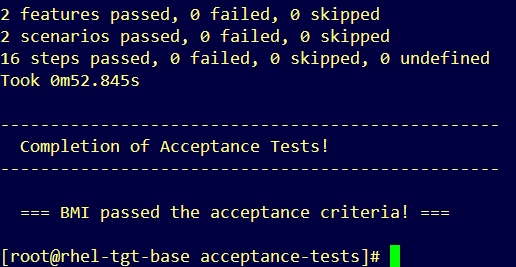
\includegraphics[scale=0.7]{figures/bdd-bmi-passed-tests.png}
\end{center}
\caption{The BMI completed successfully the end-to-end scenario}
%\label{fig:example_figure}
\label{fig:bdd-bmi-example-successful}
\end{figure}

\item To run the tests with randomized parameters, type the following where the value indicates the number of times to run the test: \\

\code{\text{}\hspace{6mm}     ./bmi-uat.py -{}-run neu-haas-dev -{}-randomize 3 } \\

\item To check if the tests passed or failed, type the following: \\

\code{\text{}\hspace{6mm}       ./bmi-uat.py check } \\

  You should see the following: \\
 
\code{\text{}\hspace{6mm}         All tests passed! } \\

  This command checks the \code{test-results} directory for any subdirectory containing \code{FAIL} in its name. \\
 
\item To cleanup all previous results, type the following: \\

\code{\text{}\hspace{6mm}       ./bmi-uat.py clean } \\

\end{enumerate}

By following the above steps you can now test your own customizations of BMI any services.
